The Toric Code is an exactly soluble spin model with $\mathbb{Z}_2$ topological order that was introduced by Alexei Kitaev \cite{cite:fault_tolerant_quantum_computation_by_anyons}. The model is defined on the square lattice with periodic boundary conditions, where on each edge of the lattice there sits a spin-1/2 degree of freedom. Two operators are introduced, the \textit{star operators}
\begin{equation}
	\label{eq:star_operator}
	A_+ \coloneqq \sum_{j\in+}\hat{\sigma}_j^z
\end{equation}
and the \textit{plaquette operators}
\begin{equation}
	\label{eq:plaquette_operator}
	A_{\scalebox{0.6}{$\square$}} \coloneqq \sum_{j\in \scalebox{0.6}{$\square$}} \hat{\sigma}_j^x,
\end{equation}
where the sums are performed over the four spins connected in a star or plaquette pattern respectively (see figure \figref{fig:toric_code_star_and_plaquette_operators}) and $\hat{\sigma}_j^x, \hat{\sigma}_j^z$ are Pauli matrices. The Hamiltonian of the Toric Code model is then defined as
\begin{equation}
	\label{eq:toric_code_hamiltonian}
	H_\text{TC} \coloneqq -\sum_+A_+ - \sum_{\scalebox{0.6}{$\square$}}B_{\scalebox{0.6}{$\square$}},
\end{equation}
where the sums go over all possible stars and plaquettes respectively. Because an arbitrary star and plaquette operator share either two or zero spins, all terms of the Hamiltonian commute and it is thus possible to find the ground state of the model by diagonalizing all terms simultaneously. One can show that the ground state up to normalization is given by the equal weighted superposition of all states that can be obtained by applying an arbitrary combination of plaquette operators to the product state $\left|\uparrow\right\rangle \otimes \dots \otimes \left|\uparrow\right\rangle$:
\begin{equation}
	\left|\Psi_0\right\rangle \propto \prod_{\scalebox{0.6}{$\square$}}\left(\id + B_{\scalebox{0.6}{$\square$}}\right) \left|\uparrow\right\rangle \otimes \dots \otimes \left|\uparrow\right\rangle.
\end{equation}
Note that this is also the ground state for the model if open boundary conditions are chosen instead. \par
For periodic boundary conditions, which is equivalent to putting the model on a torus, one can further show that the ground state is fourfold topologically degenerate. To move from one degenerate section of the Hilbert space to another a string of operators must be applied, wrapping once around the torus. This is a highly non-local operation. Because perturbarions are usually local, the toric code model can be interpreted as a form of "hardware level" error correction. The toric code is considered a topological quantum error correction code and can in theory be used for quantum "memory". One can further implement quantum gates acting on the 4-dimensional ground state space by locally creating a pair of anyonic excitations, moving one of the excitations around the torus, and annihilating it with the other one \cite{cite:fault_tolerant_quantum_computation_by_anyons}. Unfortunately, the gates that can be implemented as such do not form a complete state set and thus do not allow for universal quantum computing. Nevertheless, the Toric code is an important model for the study of topological order and anyonic excitations.
\begin{figure}
	\centering
	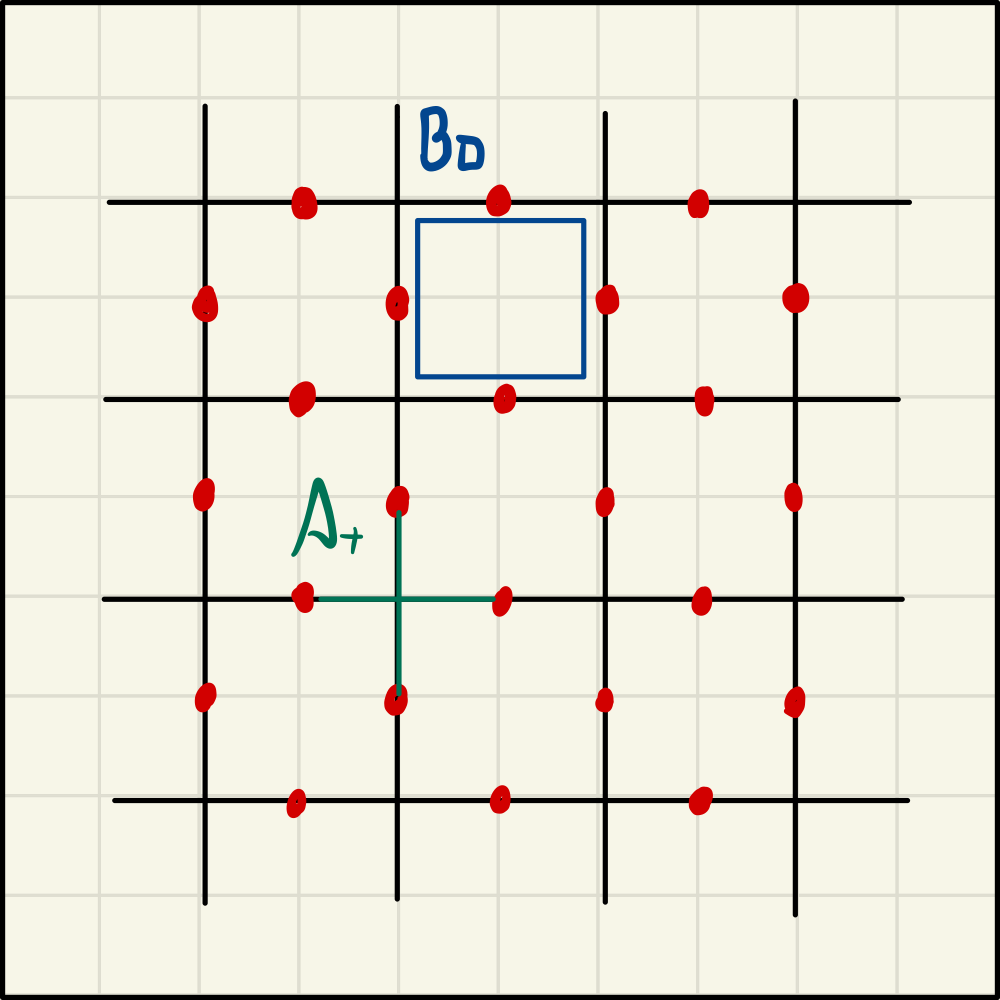
\includegraphics[width=0.6\textwidth]{figures/Toric_Code/toric_code_star_and_plaquette_operator.jpeg}
	\caption{The Toric Code model is defined on the square lattice with spin-1/2 degrees of freedom living on the edges. the star and plaquette operators \eqref{eq:star_operator} and \eqref{eq:plaquette_operator} act on the four spins aranged in a star or plaquette shape respectively.}
	\label{fig:toric_code_star_and_plaquette_operators}
\end{figure}
